%
%
%

\section{ATLAS}
ATLAS is a multi-purpose particle detector designed to identify and reconstruct particles produced in LHC collissions for primary purpose of particle discovery.
In order to fulfull this broad role, the ATLAS detector must excel in several ways simultaneously:

\begin{itemize}
  \item It must be sensitive to a wide spectrum of particle that can be produced by particle colissions, including Leptons (Electrons and Muons), Hadrons (Pions, Kaons, and the many other bound states of quarks that typically come in the form of Jets), and Photons.
  \item It must be able to identify precisely the kinematic properties of these particles, which includes measuring their energies and directions with a high resolution.
  \item It must maintain its resolution over a large range of energies, roughly from 1 GeV up to and including the TeV scale.
  \item It must make these measurements at an extremely high rate, millions of times a second, and over the entire lifetime of the experiment, which could end up being decades
  \item It must be able to record, save, and successfully distribute its collected data to experimentalists and analyzers around the world.
\end{itemize}

These requirements are entirely non-trivial, and fulfilling them required decades of design, construction, engieneering, and maintenence.  
ATLAS is a collection of many components whose various measurements are combined and merged to form a complete of a collission event.

%The original design for ATLAS
%In order to be successful, ATLAS 
%to use a wide spectrum of detector designed to discover particles and to precisely measure their proproperties.

%Typical descriptions of the ATLAS detector list its various components and describe their properties.
%But perhaps it is more useful to instead approach the detector from the perspective of the different particles that it is designed to detecct, and to use that as a springboard to go into machine's enieneering details.


\subsection{Overview}

The ATLAS detector is designed with a cylindrical geometry that supponds the LCH's beam pipe and is centered around one of the several points where proton bunches are made to collide.
The detector has a diameter of 25m, is 46m long, and weighs 7000 tonnes.
It contains about 100 million electronic channels and about 3000 km of electric cables.

\begin{figure}
  \begin{center}
    % Detector Images: http://cdsweb.cern.ch/record/1095924
    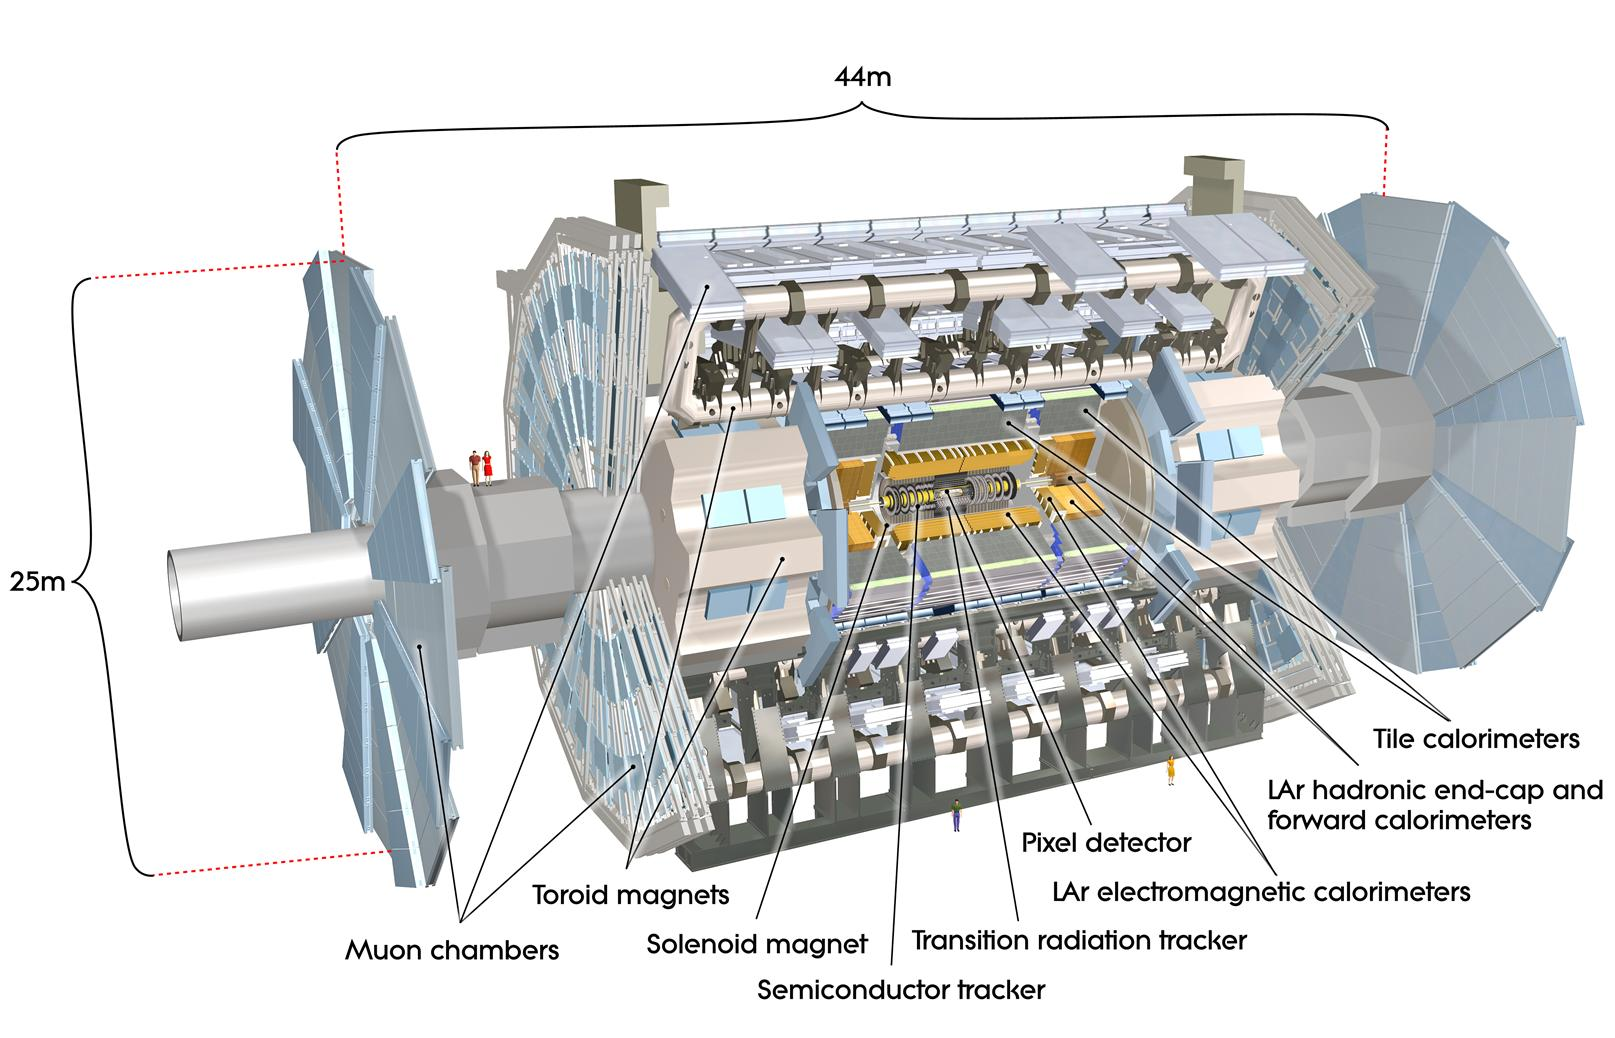
\includegraphics[width=125mm]{figures/atlas/AtlasDetecterOverview.jpg}
  \end{center}
  \caption{A schematic of the ATLAS detector showing its scale and its subcomponents.}
  \label{img:AtlasDetectorOverview}
\end{figure}

ATLAS is a multi-component detector consisting of many individual subsystems, each of which measures a certain number of kinematic properties of particles created or scattered by the LHC.
Only when combining the measurements of these sub-systems do complete pictures of particles and entire begin to emerge.
The subcomponents of ATLAS are layered around the central location of the primary interaction.
The inner-most layer of ATLAS is the ``inner detector'', which consists of silicon strips and pixils and is designed to track the 3-d trajectories of charged particles passing through it.

The inner detector extends for 1.15 m and is surronded by a solonodial magent which provides a 2T field within the inner detector.
This field causes charged particles to bend and allows the inner detector to measure the momenta of charged particles by fitting their trajectories.
Surronding the inner detector is the electromagnetic calorimeter, which consists of alternating layers of lead absorbers and active electronics that are baithed in liquid argon.
The liquid argon must of course remain cooled, and so the electromagnetic calorimeter is located within a cryostat that maintains a temperature of [XX].
To reduce the amount of upstream material present before the calorimeter systems, the solonodial magent for the inner detector is located within the EM calorimeter's cryostat.
A dedicated presampler is located directly behind the cryostat's wall to correct for any energy lost within inactive material in front of the EM calorimeter.

Behind the outside of the cyrostat and past the EM calorimeter is the hadronic calorimeter, which consists of alternating layers of iron and scintillating tile.

Finally, the outer-most layer of ATLAS is the muon spectrometer, which consists of many subsystems designed to detect the trajectories of muons at high rates and with good resolution. 
A 8T magnetic field is induced across the entire muon system and is produced by large superconducting toroid magnets.


\subsection{Geometry}
The location of ATLAS' components and the properties of identified particles are described using a common coordinate system.
One can define a right-handed euclidean coordinate system whose origin is the middle of the LHC's beam pipee in themiddle of ATLAS.
In this system, the z-direction is aligned along the beam pipe, and the x-axis points toward the center of the LHC ring.
More often, one uses a cylindrical coordinate system, which is aligned along the LHC's beam pipe.
In this system, $\phi$ referrs to the aximuthal angle around the cylander's axis of rotationall symetry, and $\theta$ is the polar angle defined such that the $\theta=0$ plane cuts the detector into two cylanders of exactly half the size.
Instead of $\theta$, it is more common to describe the polar angle in terms of the ``pseudorapidity,'' $\eta$, which is defined as $\eta = -log(tan(\frac{\theta}{2}))$
The transverse direction referrs to the radial direction in the cylindrical coordinate system 
For example, $p_{T}$ stands for the component of the momentum in the transver plane and $\met$ is the missing energy (or, more accurately, momentum) in the transverse plane.


\begin{figure}
  \begin{center}
    % Coordinate System: http://www.hep.lu.se/atlas/thesis/egede/thesis-img306.gif
    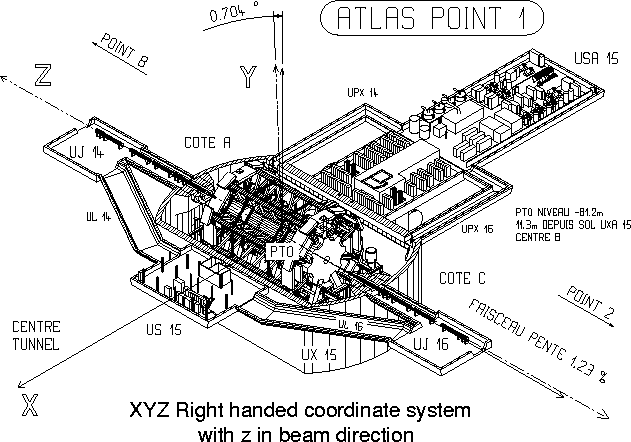
\includegraphics[width=100mm]{figures/atlas/AtlasCoordinateSystem.png}
  \end{center}
  \caption{A schematic of the euclidean coordinate system used by ATLAS.}
  \label{img:AtlasCoordinateSystem}
\end{figure}

\subsection{Inner Detector}
The inner detector is first part of the ATLAS detector encountered by particles emerging from the interaction point.
The inner detector (ID) consists of three subsystems which are designed to track the trajectories of charged particles as a collection of discrete points where they hit active parts of the detector.

\begin{figure}
  \begin{center}
    % Inner Detector: http://www.ge.infn.it/~rossi/leoweb/ID_perspective_layout.jpg
    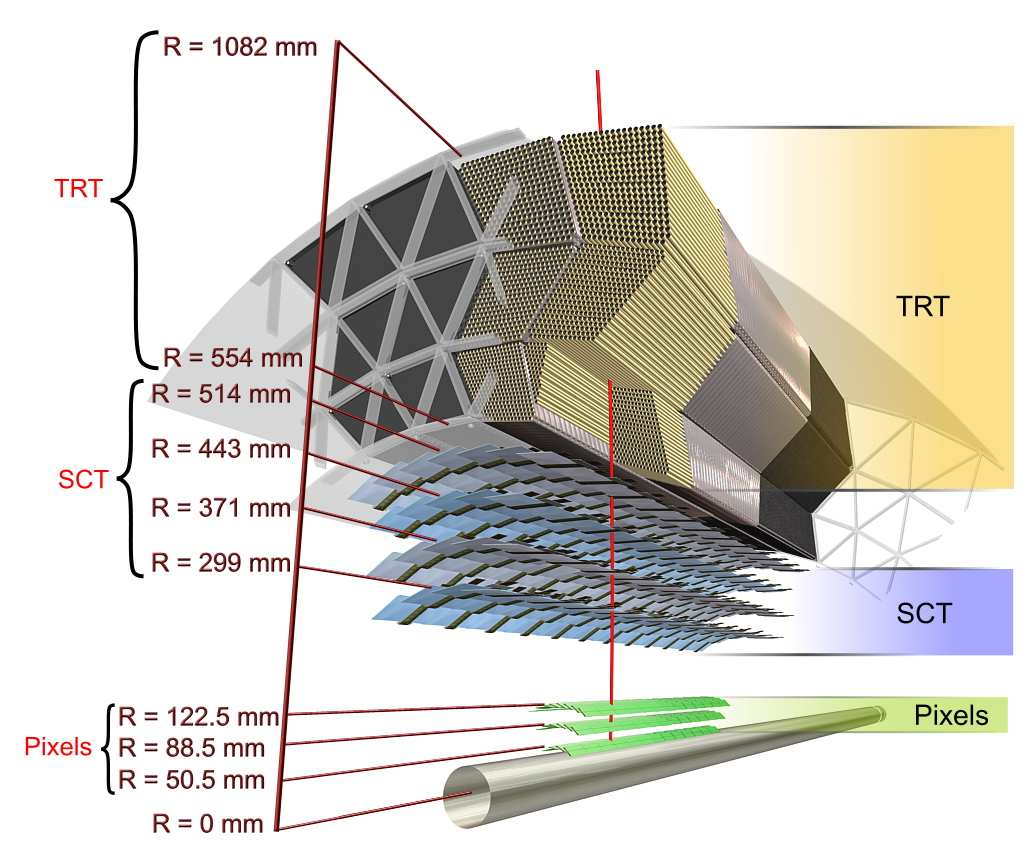
\includegraphics[width=100mm]{figures/atlas/InnerDetector.jpg}
  \end{center}
  \caption{A schematic of the ATLAS Inner Detector, showing the Pixel Detector, the Semi-Conductor Tracker, and the Transition Radiation Tracker.}
  \label{img:InnerDetector}
\end{figure}


The first layer of the ID is the pixel detector, which itself consists of three barrel layers of pixel modules at radaii of 5 cm, 10 cm, and 13 cm (on average) as well as three endcap disks on each side of the deterctor to cover the forward region in pseudorapidity.
The entire barrel cylander is 1.4 m long and .5 m in diameter.
The inner-most layer of the barrel pixel detector is known as the ``b-layer'' for its importance in the identification of displaced vertices due to b-quarks.
% The ``b-layer'' also plays an important role in separating prompt electrons from photons that convert into an electron-positron pair
(An upgrade to the detector will add an additional b-layer, known as the insertable b-layer, in space that will be freed up the beam pipe is replaced with a smaller version.)
Each region contains a collection of pixel modules (which are identical across the barrel and disk regions) which are 62.4 mm long and 21.4 mm wide.
The individual modules contain 61,440 pixel elements, and there are 1500 such modules in the barrel and 700 in the disks. %read out by 16 chips, each serving an array of 24 by 160 pixels 
In total, there are about 140 million detector elements. % each 50 μm in the Rφ direction and 300 μm in z,
The pixel detectors are designed to measure the impact parameters of short-lived particles lead to non-neglegable displaced vertices, such as $\tau$s and b-quarks.
Charged particles moving through the pixel detector will hit individual pixel diodes, which will create an electrical current that is amplified and sent to the readout system.

% Pixel Image: http://www.atlas.ch/pixel-detector.html
% Paper and individual pixel image: http://arxiv.org/pdf/physics/0412138.pdf
% Tracking performance of the pixel detector: http://www.sciencedirect.com/science/article/pii/S0168900206007157 (2004)
% B-layer upgrade (insertable, IBL): http://cdsweb.cern.ch/record/1207594/files/ATL-INDET-PROC-2009-012.pdf

Moving outward through the inner detector, the next layer encountered is the Semiconductor tracker (SCT), which is made up of several layers of silicon strips.
Since it exists at a larger radius, the SCT must cover a larger area (about 61 $m^2)$ with active material.
For the same reason, it can afford to be coarser than the pixel detector.
The SCT contains 6.2 million readout channels that are spread across four complete barrels at radii of 30.0, 37.3, 44.7 and 52.0 cm, and three rings of end-cap detectors on either side.
Each subdetector consists of a collection of 6.36$\times$6.40 $cm^2$ silicon strips (each with 768 readout strips) arranged in an overlapping pattern with each strip aligned at a small angle.
The spatial resolution is of the SCT is 16 $\mu$m in $R-\phi$ and 580 $\mu$m in z, which can distinguish tracks that are separated by as little as 200 $\mu$m.

The final component of ATLAS' inner detector is the Transition Radiation Tracker (TRT).
The TRT is designed to cover a large volume and to operate at high rates.
The TRT is a collection of thin tubes, called ``straws,'' which are 4 mm in diameter and have a maximum length of 144 cm.
Each straw has a 30 $\mu$m diameter wire at its center and is filled with a mixture of xenon gas (70\%), $CO_2$ (20\%) and $CF_{4}$ (10\%).
The entire TRT consists of a barrel section, consisting of 50000 straws running parallel to the beam axis and ranging from 56 to 107 cm in perpendicular radius from the beam pipe, and two end caps which contain 320 000 radially oriented straws.
Each straw in the barrel is divided into two readouts which are separated by an inactive middle region.
In total, there are 420,000 electronic readouts from the TRT.
As charged particles pass through a straw, they will ionize the gas, and these ions will drift toward the central wire.
The shape of the electronic pulse read out by the central wire can be used to determine the closest radius and the direction of the charged track flying through the tube.
Each straw is able to provide a spacial reolution of 170 $\mu$m.

% Should show a picture here, otherwise one one will get it  


\subsection{Electromagnetic Calorimeter}
The subcomponents that make up ATLAS's electromagnetic calorimeter are each designed to measure the energy of electrons and photons by inducing and absorbing an elecromagnetic shower.
Heavier charged particles, such as muons and pions, will interact with electromagnetic calorimeters, but their interaction lengths are longer than those of electrons and photons, which makes their showers more elongated.
As a result they do not deposit a majority of their energy within the range of ATLAS' EM calrimeters.
ATLAS' Electromagnetic calorimeter is divided into three subsections consisting of the barrel calorimeter, which covers a pseudorapidity range of $|\eta| < 1.475$ and the two end-cap calorimeters, which covers $1.375 < |\eta| < 2.5$.
However, as opposed to the hadronic calorimeter, each subcomponent shares a common design.
The calorimeter consists of layers of lead absorbers shaped in a zig-zag, accordian-like pattern and similarly arranged Kapton electrodes placed in the middle of gaps between the lead absorbers.
%The calorimeter consists of alternating layers of Kapton electrodes and lead absorbers that are both shaped in a zig-zag, accordian-like pattern.
The calorimeter's zigs and zags are aligned in the radial direction, which removes the possability of inactive cracks where two plates meet.
The entire calorimeter is bathed in liquid argon, which is maintained at a temperature of about 88 degrees kelvin by the cryostats that encases the electromagnetic calorimeters (for this reason, ATLAS' electromagnetic calorimeters are commonly referred to simply as the ``LAr calorimeter'').


\begin{figure}
\begin{center}
% http://ars.els-cdn.com/content/image/1-s2.0-S0010465511003092-gr002.jpg
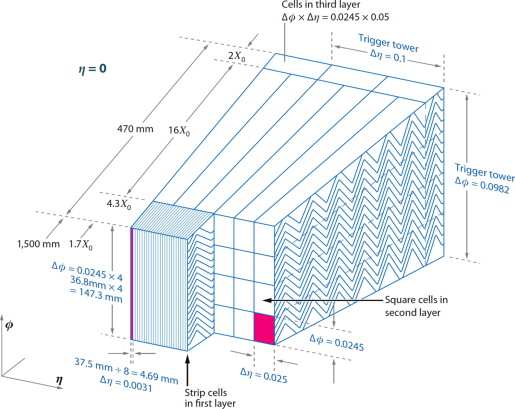
\includegraphics[width=100mm]{figures/atlas/ElectromagneticCalorimeter.jpg}
\end{center}
  \caption{A schematic of the barrel Electromagnetic calorimeter.  Shown are the three layers of the calorimeter and the accordian layout of the lead absorbers and electrodes.}
  \label{img:AtlasDetectorOverview}
\end{figure}


As charged particles fly through the calorimeter, they will ionize the Liquid Argon, and ionized electrons are drawn toward the active electrodes by a high voltage electric field (of about 1 kV/mm) that is maintained throughout the calorimeter. % [http://arxiv.org/pdf/0912.2642v4.pdf]
The current absorbed is preportional to the energy deposited, which is used to reconstruct the energy of the electron hitting the calorimeter.
Each LAr calorimeter is segmented into three or four transverse layers and is divided into cells of varying granularity in  $\Delta \eta \times \Delta \phi$, depending on the location and on the layer.%$ = 0.1 \times 0.1$ for $|\eta| < 2.5$ and up to $\Delta \eta \times \Delta \phi = 0.4 \times 0.4$. for $3.1 < |\eta| < 4.9$.
In all, the LAr calorimeter has 182,468 readout cells.
Of particular importance is the first layer of very LAr barrel calorimeter, which is finely segmented ``strips'' of  $\Delta \eta \times \Delta \phi = (0.0031 \times 0.098)$. 
This this $\eta$ segmentation allows for the resolution of the EM shower shape differences between photons and $\pi_{0}$s which decay into narrowly separated photon pairs, 
In the barrel, the three layers of LAr calorimeters have thicknesses of 4.3, 16, and 2 radiation lengths, respectively.
In addition, the barrel contains a presampler layer, which consists of LAr electrods, but no lead absorber, that is used to correct for energy lost in the inner detector, the solenoid magnet, and in the cryostat walls (the end caps have less material upstream from the EM calorimeters and therefore don't require a presampler). % [http://www.hep.lu.se/atlas/thesis/egede/thesis-node43.html]

% Helpful Talk: [http://www.physics.utoronto.ca/~krieger/talks/Krieger_NSS05_Talk.pdf]
% Commissioning ATLAS paper: [http://arxiv.org/pdf/0912.2642v4.pdf]
% LAR Temperature: [http://cdsweb.cern.ch/record/686091]


\subsection{Hadronic Calorimeter}
The Large Hadron Collider is thus named because it collides a specific hadronic bound state of quarks known as the proton.
The majority of interactions between these particles are mediated by the strong force (QCD), and the vast majority of final state particles are cone-like sprays of hadronic particles known as Jets.
It is therefore crucial that a detector working with a hadron collider be excellent at identifying and measuring hadronic particles.

% General Hadronic Calo layout
The primary means of studying a jet is through calrimetry, where the energy of a jet is determined by stopping its hadronic shower using a dense material and measuring the energy it deposits in an active material.
The direction of the jet is determined by the  $\eta$, $\phi$ location of where the jet hits the detector.
The ATLAS hadronic calorimeter is designed to contain as much of a hadronic shower within the calorimeter itself and to accurately determine its energy using the calorimeter's active components.
It is divided into three subsystems that cover overlapping ranges in pseudorapidity.
The largest and most important is the ``tile'' hadronic calorimeter (which itself is divided into the ``barrel'' and two ``extended barrel'' tile calorimeters), which covers the rapidity region of $|\eta| < 1.7$. [tdr]  
The ``hadronic end cap'' (HEC) extends the calorimeter's range up to $|\eta| < 3.2$, and the ``forward calorimeter'' (FCAL) covers the pseudorapidity range of $3.1 < |\eta| < 4.9$.  

\begin{figure}
  \begin{center}
    % http://hedberg.web.cern.ch/hedberg/home/atlas/calorimeters_9.pdf
    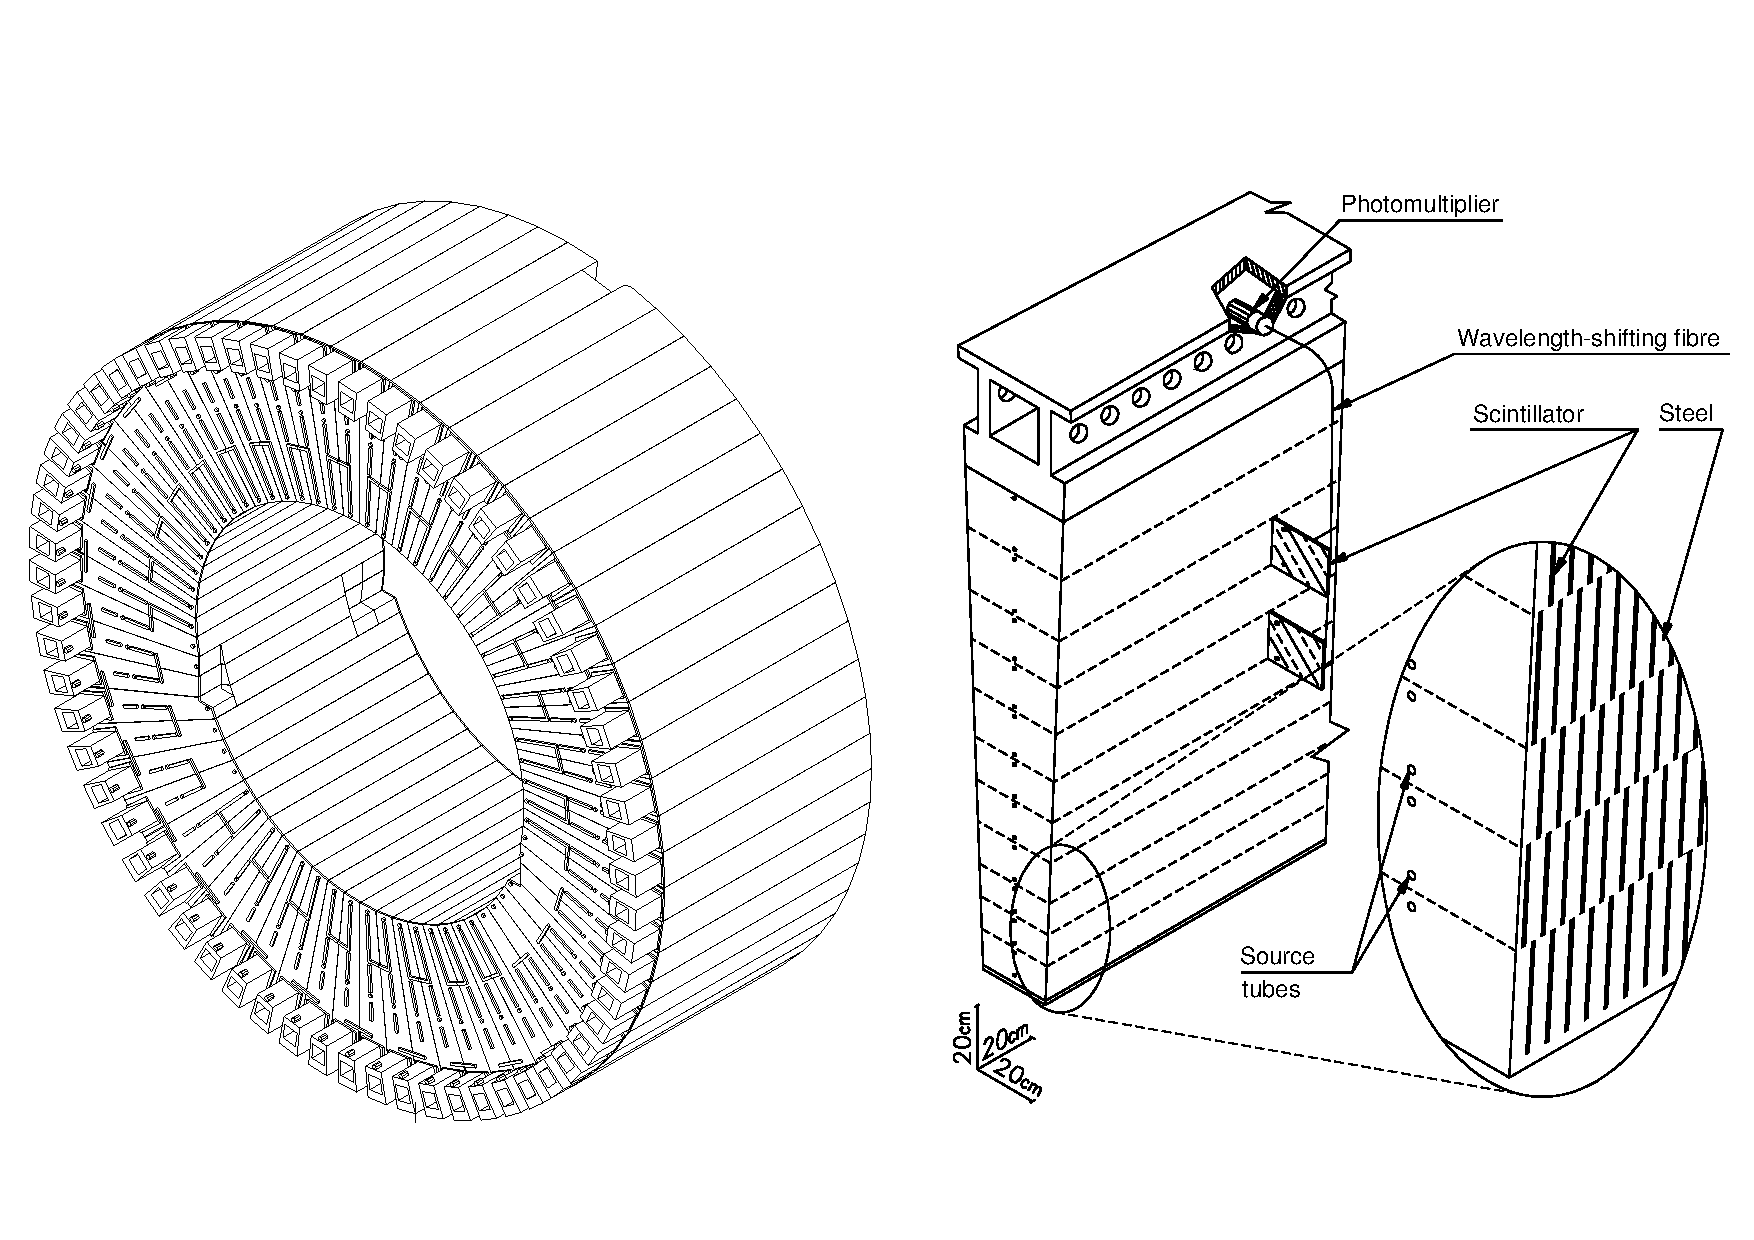
\includegraphics[width=125mm]{figures/atlas/TileCalorimeter.pdf}
  \end{center}
  \caption{A schematic of the ATLAS Hadronic (Tile) calorimeter}
  \label{img:AtlasDetectorOverview}
\end{figure}



%Each of these subsystems have similar goals but vary in their design.

% [pdg review: http://pdg.lbl.gov/2011/reviews/rpp2011-rev-passage-particles-matter.pdf]

% [http://rd11.web.cern.ch/RD11/rkb/PH14pp/node80.html]

% The Tile
The hadronic tile calorimeter, which covers [XX] starradians, detects jets that emerge low pseudorapidity, including those that are close to perpendicular to the beam pipe.
It is a cylindric shell ranging from an inner radius 2.28 meters and outer radius 4.25 meters.
The tile is made of three subsystems, one central ``barrel'' calorimeter which covers $|\eta| < 1.0$ and two ``extended barrel'' calorimeters, which cover $0.8 < |\eta| < 1.7$ on either side.
The tile calorimeters consist of alternating layers of 14 mm iron plates, which is used for inducing the hadronic shower and stopping the jet, and 3mm active scintillating-tile, which is used to measure the energy deposited into the calorimeter by the jet.
%Iron is used because the hadronic particles that make up jets interact strongly with nucleii, and therefore a material with a high nuclear density is desirable.
The scintillating tile is attached to a series of photomultiplier tubes (PMTs) that amplify the tile's electrical readout.
Key to the successful performance of the tile calorimeter is providing enough average interaction lengths for the hadronic shower to be contained.
The hadronic thickness at the end of the tile calorimeter (at $\eta=0$) is 9.2 $\lambda$, which is enough to ensure good jet resolution and to minimize jet ``punch through'' into the muon system.


\subsection{Muon Spectrometer}
The Muon spectrometer is a set of tracking chambers that cover a large volume on the outside of ATLAS that are used to determine the trajectories of Muons.
Much of the spectrometer is located within a strong magnetic field of 8 Tesla that is created by large toroidal magnets in the barrel region (which covers $|\eta| < 1.0$ as well as smaller end-cap magnets which cover the range $1.4 < |\eta| < 2.7$. 
The magnetic field in the transition region is comes from a combination of the barrel toroidal magnets and the end-cap magnets.
The muon magnet system is designed to provide a field that is mostly orthogonal to the trajectories of muons throughout the majority of the muon spectrometer.
The spectrometer itself is build out of different types of muon chambers that are designed either for precise or fast tracking measurements.
The fast chambers are mainly used for muon triggers, which must perform at the high LHC collission rate.
The precision measurements come from Monitored Drift Tubes (MDTs) and Cathode Strip Chambers (CSCs), while the trigger chambers include Resistive Plate Chambers (RPCs) and Thin Gap Chambers (TGCs).
The barrel section of the Muon spectrometer, chambers are arranged in three cylindrical layers of radaii 5, 7.5, and 10 m, covering the pseudorapidity range $|\eta| < 1$.
These layers consist of MDTs, and triggering in the barrel uses a collection of RPCs.
The end-cap chambers are aligned vertically and stacked into four disks at distances of 7, 10, 14, and 21–23m from the beam spot which collectively cover the rapidty range of $1 <|\eta|< 2.7$. 
The MDTs in the end-cap are complimented by CSC chambers which cover $|\eta| > 2$ and triggering in the end-cap is performed using TGCs.
The positioning of all chambers are actively monitored by alignment rays.

% Muon Commissioning: http://arxiv.org/pdf/1006.4384v2.pdf
% Good image on page 20

\subsection{Measuring Particles with ATLAS}


\begin{figure}
  \begin{center}
    % http://www.quantumdiaries.org/wp-content/uploads/2008/03/ce0155m.jpg
    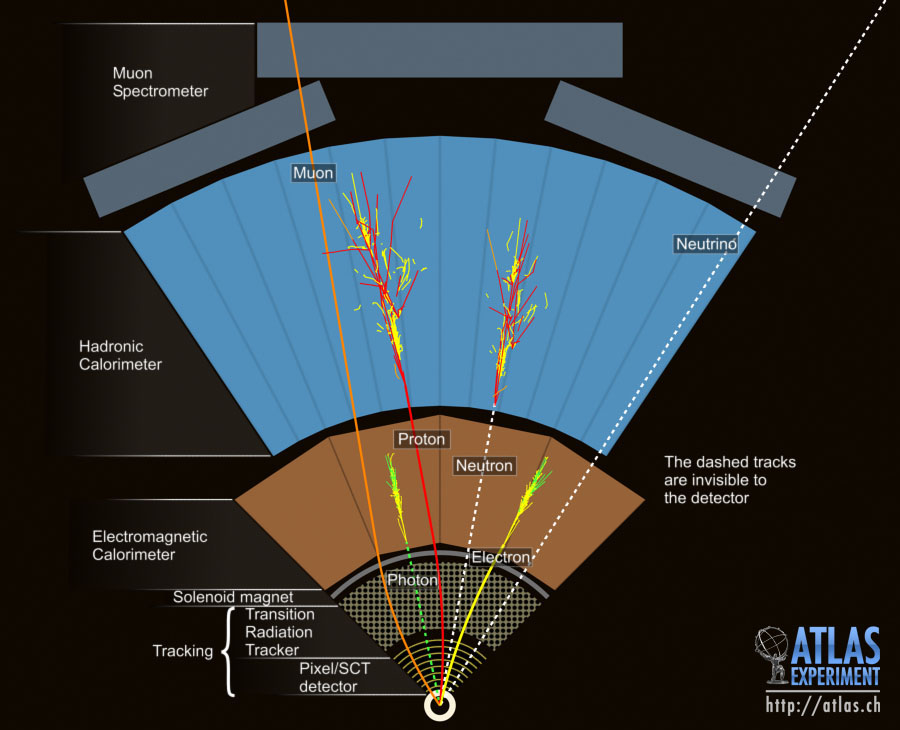
\includegraphics[width=125mm]{figures/atlas/ParticleInteractionOverview.jpg}
  \end{center}
  \caption{An overview of how various particles interact with different components of the ATLAS detector.}
  \label{img:ParticleInteractionOverview}
\end{figure}



\subsection{Jets}
Jets are produced when particles with color charge, quarks and gluons, are in the outgoing states of a hard interaction.
As these particles propogate through space, they will tend to decay into or radiate other color-charged particles, which in turn radiate and decay, leading to what is called a ``parton shower.''
This shower grows rapidly because QCD, which is an asymptotically free field theory, has a small coupling constant at high energies.  
As the shower progresses and the average energy of the constituent particles decreases, the QCD coupling constant will grow stronger, and this will cause the quarks and gluons to bind together into stable particles in a process known as ``hadronization.''
The collection of these hadrons, which move in a wide, cone-like shape, is known as a jet.
%The average distance for the parton-shower, hadronization evolution process is small compared to the radius of ATLAS, adn so jets are fully formed as they begin to interact with the detector

A jet originating from the beam spot and and moving through ATLAS will first interact with the inner detector.  Since many of the constituent particles of a jet are charged hadrons ($\pi^{+}$, $K^{+}$, etc), they will leave tracks in the ID.
Jet algorithms can use these tracks when attempting to identify a jet, and there are algorithms that exclusively rely on this collection of tracks to build a set of identified jets.
%[ Track Jets, 2009: https://atlas.web.cern.ch/Atlas/GROUPS/PHYSICS/CONFNOTES/ATLAS-CONF-2010-002 ].
However, the most common way to reconstruct jets is using the calrimetry.
Jets will deposit a small fraction of their energy in the Electromagnetic Calorimeter, but the majority of the shower's energy is measued by the hadronic calorimeter.
A small number of jets managed to escape the hadronic calorimeter and enter the muon chambers, where they can be misidentified as mouns.
In addition, jets with ``heavy flavor'' may contain decays that result in real muons (but not muons that originated from a hard collission in the beam spot), so care must be taken to separate muons originating as jets from muons originating from the hard process.

There are many algorithms used to reconstruct jets using information from the hadronic calorimeter, but most of them consist of clustering algorithms which group together cells of energy deposits.
The main differences between techniques involve how these energy deposits are calibrated (if at all) and how the cells are clustered (based on fixed geometries, such as cones, or based on iterative algorithms using a distance function to merge cell deposits).
``Cone algorithms'' are a simple category of jet clustering algorithms that use geometric cones of a fixed radius to merge energy deposits into logical jets.
An initial collection of jet candidates are collected, usually simply by selecting calorimeter deposits with energies above some threshold.
For each of these, a code is drawn of a fixed radius surronding the jet candidate (where the radius refers to the the quantity $R = \sqrt{(\Delta \eta)^2 + (\Delta \phi)^2}$) and the centroid of the transverse energy within that cone is determined.
A new cone of the same radius is drawn around that centroid, and this processes is repeated until the cone becomes stable.
Any jets that overlap must be either split and merged.
Most recent ATLAS analyses use more sophisticated techniques for clustering energy deposits to form jets.
From an initial set of preclusters, $k_T$ algorithms start by defining two sets of quantities:
\begin{itemize}
\item $d_{i} = p_{T,i}^2$
\item $d_{ij} = min(p_{T,i}^2, p_{T,j}^2)\Delta R_{ij} / D^2$
\end{itemize}
where $p_{T,i}$ is the transverse energy of a cluster, $R_{ij}$ is the distance between two clusters, and D is a fixed parameter of the algorithm 
The algorithm then proceeds by identifying the minimum $\hat{d_{i}}$ among all clusters and the minimum $\hat{d_{ij}}$ over all pairs of clusters.
If $\hat{d_{ij}} < \hat{d_{k}}$, then merge clusters i and j into a new cluster.
Else, $\hat{d_{k}} > \hat{d_{ij}}$, then cluster k becomes a jet and it is removed from the set of clusters in the algorithm.
This is repeated until all clusters are added to jets.
Anti-$k_T$ algorithms are identical to $k_T$ algorithms with the refinition: $d_{ij} = min(p_{T,i}^{-2}, p_{T,j}^{-2})\Delta R_{ij} / D^2$

% Helpful for jet algorithms:
% http://www.ccsem.infn.it/issp2009/newtalents/KPerez_Erice_JetAlgs_20090905.pdf

% How jets work, and how they shower

%% The first step in measuring a jet's energy is stopping it.  
%% The hadronic partilces that make up a jet are made up of quarks and gluons, which are charged under the strong force (QCD).
%% They therefore interact with the nucleii of materials that they pass through.
%% The primary mechanism for energy loss of high energy hadrons traveling through a solid material is via inelastic nuclear interactions.
%% As these interactions cause the original hadron to lose energy, they will also cause nuclear excitations and subsequent nuclear decays in the material.
%% This in turn leads to the emission of additional hadronic particles, which themselves will interact with the material.
%% The net effect is the formation of what is known as a hadronic shower.
%% When the energy of the daughter particles in the shower becomes too small for nuclear excitation, the shower ceases to evolve, and the remaining energy of hadrons is lost to ionization and electromagnetic interactions.
%% While the majority of energy is lost via nuclear interactions, a non-neglegable fraction of a jet's energy interacts electromagnetically .
%% This fraction 


\subsection{Electrons}
Electrons and positrons are electromagnetically charge and wil therefore interact with the innner detector, and in addition their trajectories will be curved as the particles are beant by the magnetic field.
As they pass through the inner detector, electrons will deposit hits in the pixles, silicon, and straw tubes, and the collection of these hits can be extrapolated together to reconstruct the electron's track.
This track is of crucial importance for identifying electrons.
The track carries information both about the direction of the electron, but also about its momentum, and the presence of a track is necessary to distinuish electrons from photons, which lead essentially identical electromagnetic showers in the EM calorimeter.
When electrons enter the EM calorimeter, they will begin to decellerate, which will cause the electron to radiate via bremsstralung.
The radiated photons often have enough energy to produce electorn-positron pairs, which themselves will emit bremsstralung radiation.
This creates a cascade of electrons, positrons, and photons that is collectively known as an electromagnetic shower.
The energy of this shower is determined as it is absorbed by the EM calorimeter.
The EM calorimeter tends to provide a better energy resoltion for high pT electrons than the tracks do (beginning when the electron's energy is around 10 GeV).

% [ 2010 performance: http://cdsweb.cern.ch/record/1273197 ]
% [ https://atlas.web.cern.ch/Atlas/GROUPS/PHYSICS/PUBNOTES/ATL-PHYS-PUB-2011-006/ATL-PHYS-PUB-2011-006.pdf ]
% [ Moriond 2012 Resolution info: https://indico.cern.ch/getFile.py/access?contribId=3&resId=1&materialId=slides&confId=163471]
% [ https://twiki.cern.ch/twiki/pub/AtlasProtected/EnergyScaleResolutionRecommendations/summary_rel16.pdf ]
% http://cdsweb.cern.ch/record/1209898

ATLAS employs two types of electron identification.
High pt electrons are identified using a sliding window algorithm.
Energy towers are created by adding together the energies in the four layers of the Electromagnetic calorimeter (including the presampler).
Energy deposits created by electromagnetic showers are searched for by scanning a 5$\times$5 window of these towers, and em-cluster candidates are seeded when the energy in the window is greater than 3 GeV.
A 3$\times$7 cluster is then formed using the middle layer of the EM calorimeter, and the energy of the cluster determined as the sum of the energies in the calorimeter layers in that window, including a number of corrections based on the calorimeter layer and the position in the detector.
Once an electromagnetic cluster has been identified, an attempt is made to match it to an inner detector track.
Tracks are extrapolated both to the electromagnetic calorimeter's (the first layer) and to the physical center, and ID tracks are matches to calorimeter clusters if $|\Delta \eta_{track, strips}| < 0.05$ and $-.1 < sign(q)*\Delta \phi_{track, middle} < 0.05$.
Electromagnetic clusters matching an inner detector track are considered electron candidates, which are then subject to further requirements on the electron properties, including the shape of its electromagnetic shower, its distribution within the calorimeter, and the types of inner detector hits that make up its track.

% Sliding window description:
% https://twiki.cern.ch/twiki/bin/viewauth/Atlas/SlidingWindowClustering

% ATLAS: Electron Reconstruction and Identification CSC
% http://www.physics.smu.edu/web/research/preprints/SMU-HEP-08-21.pdf

% Electron Reco:
% http://www-atlas.lbl.gov/physics/Ron_Atlas_EMID.pdf


\subsection{Photons}
Photons are identified as electromagnetic showers that aren't matched to an inner detector track.
In addition, photons may decay into an electron-positron pair before entering the EM calorimeter.
If this occurs within or before the inner-detector, the proximity of the electron and positron's tracks can be used to identify the pair as a photon that ``converted'' electromagnetically, and the pair can be reconstructed as a single photon.
Electromagnetic showers created by photons are selected in exactly the same way as those which are used to reconstruct electrons, but the requirement on a matching inner detector track is waived.  
However, photons that convert into an electron-positron pair will often be identified as electron candidates, and special care must be taken to identify those electron candidates which mostly likely originated as photons.
First, the inner detector searches for conversion vertex candidates, which are two track vertices that are displaced from the impact point where one or both tracks match an electromagnetic cluster.
For each vertex candidate, a fit is performed between the vertex, its tracks, and the matched electromagnetic clusters, using the assumption that the photon is massless.

% Photon ID and good description of conversions
% http://cdsweb.cern.ch/record/1345329/files/ATL-PHYS-PUB-2011-007.pdf

% Expected performance of the Atlas Experiment 
% (Reconstruction of Photon Conversions is: pp. 112–140 )
% http://arxiv.org/abs/0901.0512

% In addition, photons may be identified as electron-positron pairs from ``conversions,'' which are electron-positron pairs that 


\subsection{Muons}
Muons, with a mass of 106 MeV, weigh about 200 times more than the electron (which weights .512 MeV).
This implies that, for a fixed energy, a muon will have a smaller value of $\beta$ than an electron (or, equivalantly $\gamma$), which results in a smaller amount of radiation being emitted as it passes through matter.
Therefore, a muon's mean radiation length in ATLAS' calorimeters will be much longer than an electron's length, and a significant EM shower will not develop within the detector.
For this reason, most of a muon's energy escapes ATLAS' calorimeters.
As a result, the direction and momentum of muons are measured based on the direction and bending of their tracks in magnetic fields.
Muons are tracked both by the inner detector and the muon spectrometer, both of which contain large magnetic fields that bend their trajectory.
There are two main categories of muon reconstruction algorithms, but they both involve creating trajectories in both the inner detector and muon spectrometer, and matching the two to form a ``combined'' muon tractory.
``Muid'' muons use the Moore algorithm to build ``stand alone'' tracks in the muon spectrometer, which are built out of muon segments in individual drift chambers, and ``Staco'' muons build stand alone tracks using the Muonboy algorithm.
Both algorithms then perform a backward track extrapolation from the muon spectrometer to the inner detector, taking into account the magnetic field throughout the detector and energy loss from as muons travel through material.
 
% Muon id algorithms: http://cdsweb.cern.ch/record/1209632/files/ATL-PHYS-PROC-2009-113.pdf?version=1
% staco vs muid, 
% moore vs muboy

%Instead, a large volume of ATLAS' active detectors are dedicated to measuring the direction and momentum of muons my tracking their positions as they bend through a large magnetic field.
% [ pdg: Muons through matter: http://pdg.lbl.gov/2000/passagerpp.pdf fig 23.1 ]
%Since one can not measure its energy through calrimetry, ATLAS instead measures its momentum by estimating its curvature when bent in a magnetic field.
%The bending of a Muon's track in the inner detector in the magnetic field created by the solenoid can be used to determine its momentum.
%However, muons with large pt will have nearly straight tracks, which will degrade the pt resolution that can be obtained from the inner detecter alone.

% magnet can be used to  will create a bent track in the inner detector that can be used to estimate its momentum.
% However, the resolution of the inner detector for high pt muons becomes somewhat poor.
% To vastly improve on the measurement of the inner detector alone, ATLAS has a large set of detectors that comprise the muon spectrometer.
